\section{Efekt pogłosu}

Doświadczenia w~wykorzystywaniu bloków BRAM nabyte w~czasie implementacji generatora funkcji sinus pozwoliły na sprawną realizację kolejnego z~zaplanowanych efektów - pogłosu. Prace nad nim rozpoczęto od zaimplementowania parametryzowalnego \textbf{modułu opóźnienia}, ktory miał zostać użyty również w~przypadku kolejnego efektu. Zasada jego działania jest stosunkowo prosta i~zasadza się na sekwencyjnym zapisie próbek wejściowych w~pamięci RAM - traktowanej jako bufor kołowy - oraz odczycie próbek spod adresu będącego wynikiem odejmowania adresu aktualnie zapisywanej próbki i~parametru zewnętrznego (stopnia opóźnienia). Blok ten implementuje wyjście i~wejście danych oraz długości opóźnienia. Port \verb|busy| informuje o~możliwości odebrania opóźnionej próbki z~wyjścia. Wejście \verb |enable| umożlwia rozpoczęcie przetwarzenia próbki. Jego strukturę zewnętrzną przedstawiono na Rys. \ref{delay-line-structure}.

\vspace{0.5cm}
\begin{figure}[ht]
    \centering
    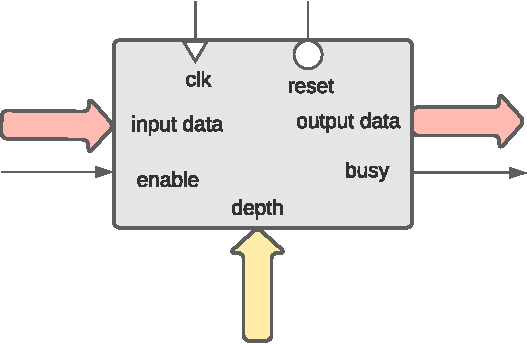
\includegraphics[scale=0.75]{img/diagrams/delay_line.pdf}
    \captionsetup{format=plain,justification=centering}
    \caption{Struktura wyprowadzeń modułu opóźniającego}
    \label{delay-line-structure}
\end{figure}
\vspace{0.5cm}

Porty bloku efektu zostały z~kolei ukazane na Rys. \ref{delay-structure}. Posiada dwa wejścia określające kolejno głębokość echa (\verb|depth|) oraz jego siłę (\verb|delay|). Pierwszy parametr interpretowany jest jako opóźnienie próbki odczytywanej z~bloku opóźniającego. Z~kolei drugi traktowany jest jako liczba z~zakresu $[0,0.5)$ przez którą mnożone jest wyjście bloku opóźniającego przed zsumowaniem go z~aktualną próbką wejściową.

\vspace{0.5cm}
\begin{figure}[ht]
    \centering
    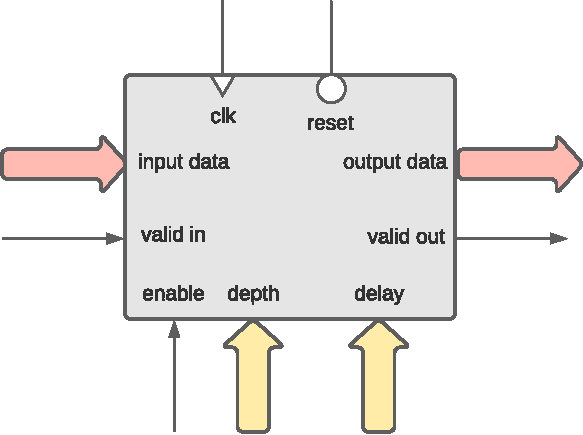
\includegraphics[scale=0.75]{img/diagrams/delay.pdf}
    \captionsetup{format=plain,justification=centering}
    \caption{Struktura wyprowadzeń bloku \textit{delay}}
    \label{delay-structure}
\end{figure}
\vspace{0.5cm}

Dzięki wydzieleniu większego elementu efektu w~postaci odrębnego bloku funkcjonalnego, proces dalszej jego realizacji był znacznie ułatwiony. Logika modułu sprowadzona została do dwustanowego automat skońćzony. W~stanie \textit{idle} oczekuje on na pojawienie się jedynki logicznej na porcie \verb|valid in|. Gdy zostanie ona wykryta, wartości z~portów danych oraz parametrów są przepisywane do wewnętrznych buforów. Jednocześnie stan wyjścia \verb|busy| efektu oraz linii \verb|enable| modułu opóźniającego ustawiany jest na wysoki. Wejście danych modułu podłączone jest na stałe do bufora \textbf{wyjściowego} efektu co oznacza, że w~pamięci BRAM zapisana zostanie próbka wynikowa \textbf{poprzedniego cyklu przetwarzania}. Po uruchomieniu bloku opóźnienia moduł przechodzi do stanu oczekiwania na wynik. Jego pojawienie się na wyjściu bloku sygnalizowane jest przez opadające zbocze portu \verb|busy|. W~momencie jego wykrycia aktualizowany jest stan bufora danych wyjściowych. W~zależności od tego czy zbuforowana wartość parametru \verb|depth| jest zerowa czy nie, na wyjście trafia nieprzetworzona wersja danych wyjściowych lub wynik (asynchronicznego) dodawania zawartości bufora wejściowego i~iloczynu wyjścia z~bloku opóźniającego z~wartością bufora \verb|delay|\footnote{Wynik iloczynu jest przesunięty w~prawo o~liczbę bitów o~jeden większą niż szerokość wejścia \textit{depth}}. Dodawanie odbywa się z~nasyceniem w~zakresie reprezentacji. Warto dodać, że blok opóźniający posiada (opcjonalną) funkcję miękkiego startu, która ogranicza wartość realizowanego opóźnienia do ilości próbek zapisanych w~pamięci BRAM od ostatneigo resetu. Ma ona na celu zredukowanie potencjalnych zniekształceń sygnału na początku działania efektów wynikajacych z~wykorzystania niezainicjalizowanych komórek pamięci jako właściwych danych.

Do realizacji bloku opóźniającego w~przypadku efektu \textit{delay} wykorzystano 21 bloków RAM, których łączna pojemność umożliwi przechowanie do $45056$ 16-bitowych próbek danych. Dla częstotliwości próbkowania na poziomie 44100Hz oznacza to możliwość osiągnięcia opóźnień rzędu jednej sekundy. Ze względu na zastosowanie bufora na wyjściu bloku BRAM opóźnienie efektu wynosi \textbf{4~cykle}. Analogicznie do przypadku poprzednich efektów celem weryfikacji poprawności działania modułu skonstruowany został projekt symulacji umożliwiający realizację różnych scenariuszy testowych. Rys. \ref{sim-delay} przedstawia fragment symulacji, w~której wartość opóźnienia została ustalona na poziomie 255 próbek, natomiast jego siła miała wartość maksymalną ($0.5$). Sygnał wejściowy to ponownie fala sinusoidalna o~częstotliwości $440$Hz próbkowana z~częstotliwośicą $44100$Hz. Jak widać włączenie efektu nie powoduje natychmiastowej zmiany charakteru sygnału. Zmiana ta następuje po czasie około $5.8$ ms. Zgadza się to z~przewidywaniami teoretycznymi ($1s / 44100 \times 255 \approx 5.8 ms$). Ponadto symulacja ukazuje zmniejszenie amplitudy sygnału po dodaniu do niego składnika opóźnionego. To również zgadza się z~przewidywaniami. Opóźnienie $255$ próbek odpowiada nieznacznie ponad $2.5$ okresom sygnału wejściowego. Oznacza to, że znaki próbki wejściowej i~opóźnionej są względem siebie odwrócone przez większość czasu, co powoduje efektywne zredukowanie amplitudy fali wyjściowej.

\vspace{0.5cm}
\begin{figure}[ht]
    \centering
    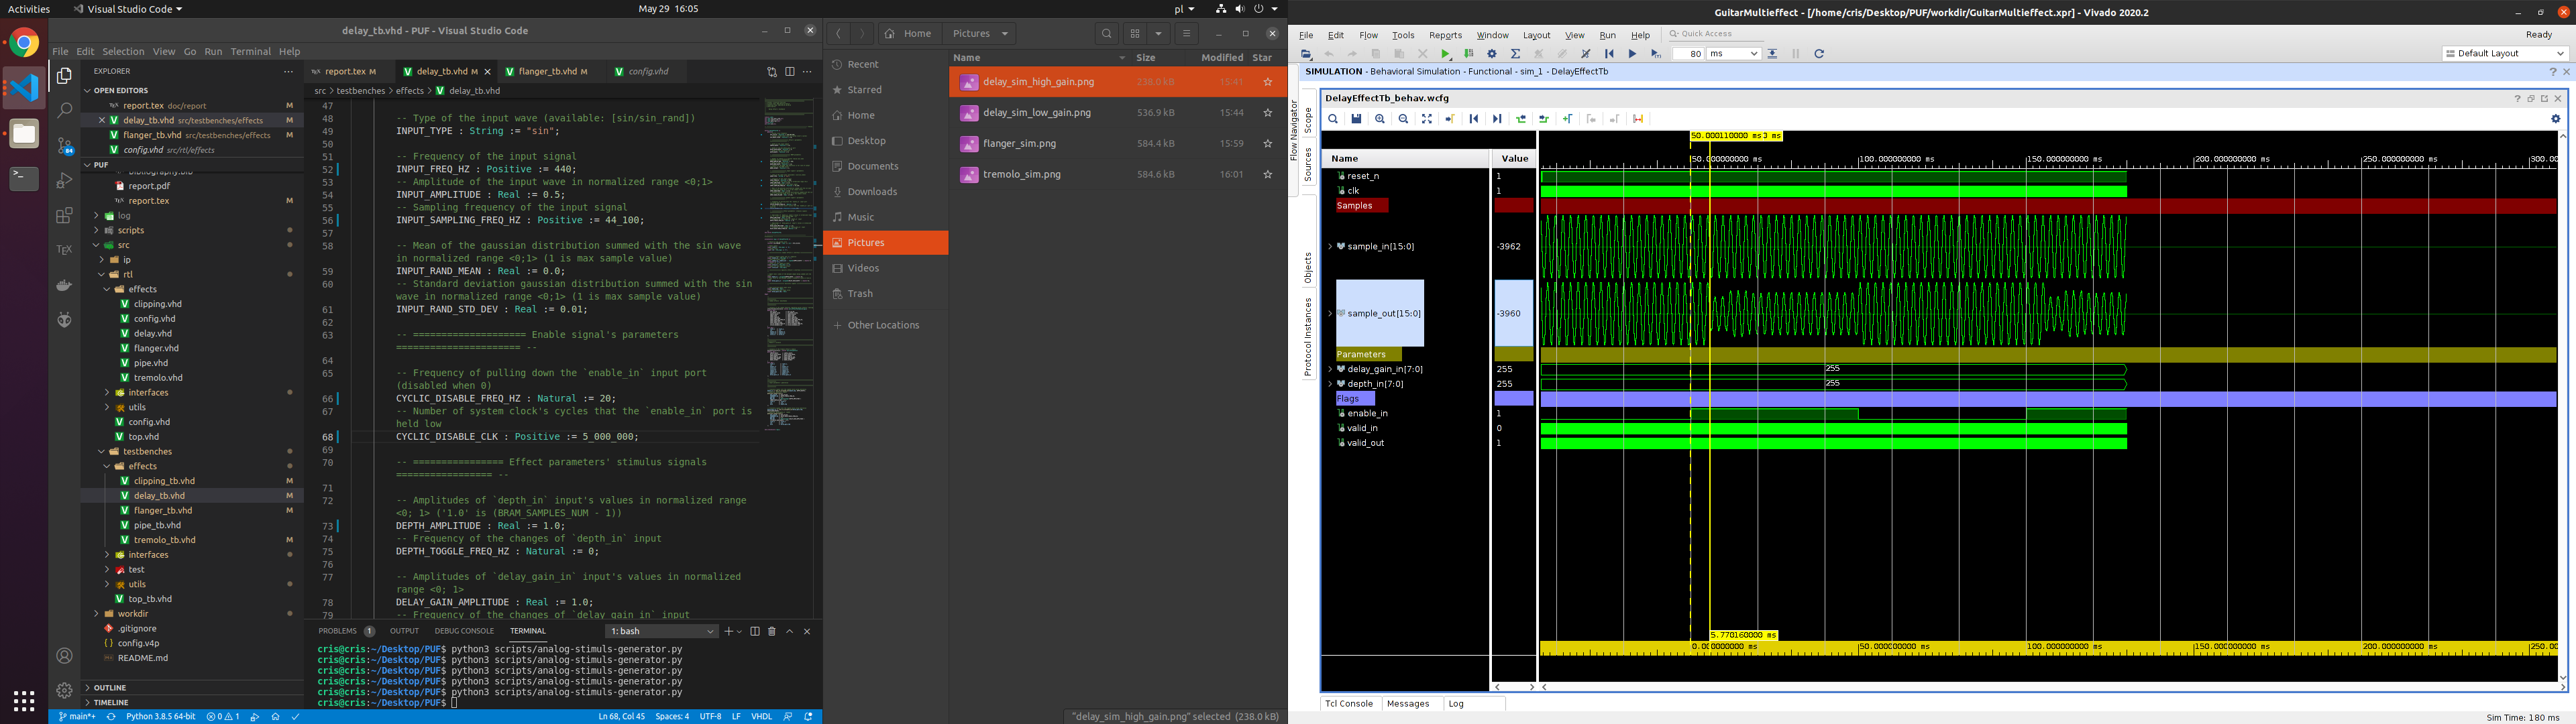
\includegraphics[width=\textwidth]{img/sim/delay_sim_high_gain.png}
    \captionsetup{format=plain,justification=centering}
    \caption{Fragment symulacji działania efektu \textit{delay}}
    \label{sim-delay}
\end{figure}
\vspace{0.5cm}